\chapter{Rain or rock? Sensitivity of a flood-inundation model to rainfall distribution and erosional parameterisation}
\label{chapter_flood_model_sensitivity}
\chaptermark{Rain or rock?}
%\begin{chapquote}{Lewis Carroll, \textit{Alice in Wonderland}}
%``Begin at the beginning,'' the King said, gravely, ``and go on till you
%come to an end; then stop.''
%\end{chapquote}

%\begin{abstract}
%Landscapes evolve and take their shape from the cumulative effect of `geomorphically effective' events. In temperate climates, these are rainfall-driven events of sufficient magnitude to trigger threshold-dependent erosional processes. This chapter investigates the sensitivity of two end-member erosional models to the spatial resolution of rainfall input to a catchment using three historic severe rainfall events in Northern England and Cornwall.
%
%It is demonstrated that the erosional model chosen exerts first-order control of the total amount of landscape change and sediment flux. However, both end member models show sensitivity to the spatial resolution of rainfall input data during individual, formative rainfall events. 
%
%\end{abstract}
\section{Introduction}

Patterns of rainfall distribution across a catchment can affect hydrograph response, including the peak discharge and local water levels (Nicotina et al., 2008). As many geomorphic processes are threshold dependent (Schumm, 1979), such as fluvial incision into bedrock (Sklar and Dietrich, 2001; Snyder et al., 2003), there is potential for the spatial distribution of rainfall to control local erosion rates within a catchment. Non-linearity in geomorphic process laws (e.g. Coulthard et al., 1998; Phillips, 2003; Coulthard and Van de Wiel, 2007) should dictate that catchments are also geomorphically sensitive to the spatial distribution of rainfall. 

The following questions are explored through the use of numerical modelling simulations;

\begin{itemize}
\item Are predicted flood inundation extents during a storm sensitive to the spatial resolution of rainfall inputs to the catchment?
\item Are fluvial erosion and sediment transport processes controls on predicted flood inundation extents in a catchment during a single severe storm.
\item Does geomorphic change of the floodplain and channel during a storm event significant enough to affect flood inundation predictions?
\end{itemize}

%%%%%%%%%%%%%%%%
\section{Experiment Design \& Method}
%%%%%%%%%%%%%%%%
An ensemble of simulations was designed to address the questions laid out in the previous section. The simulations were parametrised with different erosion law schemes and different rainfall input resolutions to assess which environmental factors exerted the greatest control over catchment response to intense rainfall, in terms of flood inundation and sediment transport. The same ensemble of experiments was carried out for two historic rainfall events that lead to severe flooding in UK river catchments. The summary of the ensemble events is given in the table below:

\begin{table}
\begin{tabular}{lll}
\\
\textbf{Experiment name}   & \textbf{Rainfall input} & \textbf{Erosion law}  \\
\hline \
UNIFORM\_HYDRO  &  Spatially averaged   & (no erosion) \\
UNIFORM\_DLIM      &  Spatially averaged   & Detachment-limited \\
UNIFORM\_TLIM       &  Spatially averaged   & Transport-limited \\

GRIDDED\_HYDRO  &  1km Gridded   & (no erosion) \\
GRIDDED\_DLIM      &  1km Gridded  & Detachment-limited \\
GRIDDED\_TLIM       &  1km Gridded   & Transport-limited \\
\hline \\ 
\end{tabular} 
\caption{Outline of the ensemble simulations carried for all case studies.}
\label{table_ensemble_experiments}
\end{table}

The numerical landscape evolution model, HAIL-CAESAR (described in Chapter \ref{chapter_HAIL-CAESAR}) is used to investigate landscape and hydrological response to varying rainfall input resolution. HAIL-CAESAR is a hydrodynamic landscape evolution model that uses a TOPMODEL-based hydrological rainfall-runoff model to generate surface runoff in a river catchment, which is then routed through the landscape according to an adaptation of the LISFLOOD-FP shallow water routing algorithms \citep{bates2010simple}. Fluvial erosion and sediment transport is then derived using the velocities and depths of the calculated surface water within the catchment. The equations describing the water routing, sediment erosion, and transport laws are described fully in Chapter \ref{chapter_HAIL-CAESAR}.


%\subsection{Rainfall-runoff and flow routing}
%From rainfall input, runoff is calculated using an adaptation of the Beven and Kirby (1979) TOPMODEL. Total surface and subsurface discharge is given by:
%
%\begin{equation}
%Q_{tot} = \frac{m}{T}\log \left( \frac{(r - j_t) + j_t \exp \left( \frac{rT}{m} \right) }{r} \right)
%\end{equation}
%
%where \(T\) is the time step in seconds, \(r\) is the rainfall rate, \(j_t\) is a function that describes soil moisture store, and \(m\) is a parameter that controls the rise and fall of this soil moisture store in \(j_t\). These adapted TOPMODEL equations are given fully in Coulthard (2002), equations (1) and (2).
%
%The amount of water partitioned between surface and subsurface flow is determined by a simple infiltration threshold, given by:
%
%\begin{equation}
%I_t = KS(Dx)^2
%\end{equation}
%
%where \(K\) is hydraulic conductivity, \(S\) is the slope, and \(Dx\) is the width of the grid cell or horizontal grid spacing. The infiltration threshold is subtracted from \(Q_{tot}\) to give the portion of water routed over the surface.
%
%Surface water and channel flow is an important driver in catchment scale erosional processes. The amount and velocity of water flow is a variable in both the sediment transport and bedrock erosion laws. The water flow equations are based on a simplified form of the shallow water flow equations, a simplification first derived by Bates (2010) and incorporated into the landscape evolution model by Coulthard et al (2013). The flow between cells is calculated by:
%
%\begin{equation}
%Q = \frac{q - g h_{flow} \Delta T \frac{\Delta (h+z) }{\Delta x}}{1 + g h_{flow} \Delta t n^2 |q| / h_{flow}^{10/3}} \Delta x
%\end{equation}
%
%where \(q\) is the water flux between cells from the previous iteration, \(g\) is acceleration due to gravity, \(h_{flow}\) is the maximum depth of flow between cells (m), \(t\) is time (s), \(h\) is depth of water, \(z\) is elevation, \(x\) is the grid well width, and \(n\) is Manning's roughness coefficient. The full implementation details are given in Coulthard (2013), and the derivation from the shallow water equations is given in Bates (2010).
%
%\subsection{Sediment transport}
%Transport of loose sediment within the model is governed by the \citet{Wilcock2003} sediment transport model. The Wilcock and Crowe model represents transport of mixed sand/gravel fractions based on the surface sediment composition. The rate of sediment transport, \(q_i\), is given as:
%
%\begin{equation}
%q_i = \frac{F_i {U_*}^3 {W_i}^*}{(s -1) g}
%\end{equation}
%
%where \(F_i\) is the fractional volume of sediment, for a given sediment fraction, \(i\), \(U^*\) is the shear velocity, \(s\) is the ratio of sediment to water density. \({W_i}^*\) is a function relating fractional transport rate to total transport rate (see \citet{Wilcock2003} for a full derivation of this equation). The usage of this sediment transport model is extrapolated here to account for finer particles such as silts \citep{Vandewiel2007}, as well as the sand-gravel mixture it was originally designed for.
%
%\subsection{Bedrock incision}
%\label{bedrock_model}
%A simple model of bedrock incision based on the excess shear stress model (Citations) is implemented in the numerical model. The rate of bedrock incision is determined by the amount of shear stress acting on the bedrock, above a threshold level of stress required to initiate substrate removal (e.g. \citet{Snyder2003}. When bedrock material is removed, it is distributed amongst the sediment fractions according to the fractional proportions set by the user. The rate of bedrock erosion according to the excess shear stress model is given by:
%
%\begin{equation}
%\varepsilon = k_e(\tau_b - \tau_c)^{P_b}
%\end{equation}
%
%where \(k_e\) is the bedrock erodibility coefficient, \(\tau_b\) is the basal shear stress on the channel bed, \(\tau_c\), is the critical shear stress threshold, \(P_b\) is the shear stress exponent. (Cite Howard or Whipple?)

%%%%%%%%%%%%%%%%%%%%%%%%%%%%%
\subsection{Study area}
%%%%%%%%%%%%%%%%%%%%%%%%%%%%%
\subsubsection{Overview}
Three upland catchments in the UK were selected to represent a range of catchment sizes and shapes. The catchments were also chosen on the basis that they had experienced a severe rain storm which could be used as a basis for the experiments, such that it could be considered `extreme' in the typical return period of flooding events for each particular catchment. Peak discharges for each of the following flood events exceed the 99th percentile for their respective catchments. The catchments and respective severe rain events chosen were located in: Ryedale, North Yorkshire, 2005; Eden, Cumbria 2012; and Boscastle, Cornwall, 2004. An overview map of their locations is given in Figure \ref{overview_fig}. A table (Table \ref{met_setting}) summarises the key features of each catchment and associated storm.

\linespread{1.5}
\begin{table}
\resizebox{\textwidth}{!}
{%
\begin{tabular}{l c c} \hline

Catchment Name 			& \textbf{Ryedale} &  \textbf{Valency} \\ \hline
Catchment Area   			& 270km$^2$ 				& 18km$^2$ \\ 
Catchment Type         & Upland, Moor/Peaty & Upland, Pasture \\ 
Storm Date	 		            & 2005-06-19 	& 2004-08-16 \\ 
Peak Rainfall	 (mm hr \(^{-1}\))  & 125  & c.400 \\
Peak Discharge	 	 & & \\ 
Meteorological Setting	 	& Split-front, convective system & Quasi-stationary convective system \\ 
3hr Rainfall Return Period 	 & 330yr (Wass et al. 2008)	& 1300yr (Burt, 2005) \\ \hline
\end{tabular}
}
\caption{Table showing key characteristics of each storm event.}
\label{met_setting}
\end{table}

\subsection{Hydro-Meteorological conditions}

\subsubsection{Boscastle, Cornwall storm 2004}
The Boscastle storm took place on the 16th August 2004 leading to flooding within the River Valency catchment and the village of Boscastle. In the preceding months March--June, the south-west region had been drier than usual, but during July the Valency catchment area experienced average rainfall conditions \citep{golding2005boscastle}. The estimated soil moisture deficit\footnote{The amount of water needed to bring the soil back to field capacity, i.e. a state where the soil is holding the maximum amount of water possible against gravity. \citep{beven2011rainfall}} in the area, which had been lower than average due to the dry antecedent conditions, decreased during the period of 1--16th August, due to the return to average rainfall conditions in that month. The soil moisture deficit during this period was estimated to have decreased from approximately 80--220mm to 40--180mm.

On the day of the storm, the extreme rainfall accumulations of up to 200 mm in the upper Valency catchment resulted from prolonged rainfall between the hours of 1200 -- 1600 UTC. Rainfall rates were thought to have reached almost 400 mm hr\(^{-1}\) \citep{Golding2006}, after correcting for under-reporting from rain gauges in the vicinity of the catchment. (Burt, 2006).

The meteorological conditions that enabled such prolonged heavy rainfall were a combination of large-scale synoptic conditions moving in from the Atlantic, with moist lower atmospheric layers readily forming convective cloud. Repeated initiation of convection along the north Cornish coast lead to what appeared to be relative stationary convective cells over the Valency catchment. Later authors refer to this type of convective storm as a `Boscastle-type' or quasi-stationary convective storm \citep{warren2014boscastle}.



\subsubsection{Ryedale, North York Moors storm 2005}
The Ryedale storm occurred on 19 June 2005. Intense rainfall throughout the afternoon lead to total accumulated rainfall amounts of up to 89mm in the Ryedale valley, between the hours of 1400 -- 1800 UTC. Peak instantaneous rainfall rates were estimated to have been around 32.5mm hr\(^-1\) (Sibley et al., 2009) to 59.4 mm hr \(^{-1}\) (Hopkins et al. 2010), though one report states they reached as high as 125 mm hr \(^{-1}\) (Cinderley, 2005). The antecedent conditions had been dry for a prolonged spell, leading to cracking of the surface peat in the higher elevations of the catchment.

Antecedent conditions before the Ryedale storm of 2005 had been dry over a prolonged period over much of the region \citep{sibley2009analysis}. Soil moisture deficit was estimated to be around 60mm in the catchmnet, higher than usual due to the drier conditions in the preceding months \citep{wass2008investigation}. With a low soil moisture content, thinner soils in the upper reaches of the catchment would have been dry before the intense rainfall.

The meteorological conditions leading to such heavy rainfall was a combination of a cold, upper-level air mass advecting over a warm moist boundary layer, leading to unstable conditions that enabled a convective thunderstorm to develop in the late afternoon. The instability was enhanced by a split-frontal system. [More? Too much met here?]. The conditions let to a particularly high amount of precipitable water present in the atmosphere which was subsequently washed out into the landscape during intense rainfall. 

\subsection{Numerical model configuration}

\subsubsection{Model initialisation}

The simulations are set to begin 24 hours before the day of each intense rainfall event. The model is allowed to run for a further 24 hours after the event, giving a total simulation tme of 72 hours. The timing of the simulations is given in Table \ref{table_start_time_hydrog_sims}.

\begin{table}[htbp]
\begin{tabular}{l c  c}
\textbf{Event}  &   \textbf{Start time} &  \textbf{End time} \\
\hline 
Boscastle          &  2004-08-15 00:00  &  2004-08-17 23:59 \\
Ryedale             &  2005-06-18 00:00  &  2005-06-20 23:59 \\

\end{tabular}
\caption{Start and end times (UTC) for each 72 simulation. The major rainfall event occurs during the 2nd day in each simulation.}
\label{table_start_time_hydrog_sims}
\end{table}

\subsubsection{Erosion model choice}
A variety of erosion laws exist describing how landscapes erode from fluvial incision. The choice of erosion law for a given catchment depends on a variety of factors, such as the characteristic substrate material in the catchment -- is it predominantly loose sediment or cohesive, solid bedrock? In reality, landscapes are often a mixture of these two extremes, incorporating loose sediment on top of solid bedrock. Catchments also often exhibit a transition from rockier upland headwaters, to more thickly soil-mantled flood plains. In order to address the uncertainty in choosing which erosion model applies for each catchment (Section \ref{theory}), two erosion model end-members are used, with each one representing a different conceptual model of fluvial incision and sediment transport. These include: i) a purely sediment transport-limited model, ii) a detachment-limited bedrock incision model. The equations describing the transport-limited and detachment-limited models are discussed in Section \ref{theory}. Further models were considered, such as a hybrid transport-detachment limited erosion model, but it was deemed beyond the scope of this study, which is to focus on the sensitivity of rainfall resolution, rather than wide range of erosion and sediment transport models. 

A set of control simulations parameterising only runoff and surface water routing (no erosion taking place) were also carried out for comparison against the two erosion end-member simulations. (Table \ref{table_ensemble_experiments}.)

%\paragraph*{Hybrid model}
%The hybrid model assumes a limited-depth sediment layer, overlying a bedrock layer. Figure \ref{hybrid_model} shows a typical cross section through a typical valley in the hybrid model set-up. In the initial model state (before the spin-up period), a channel is 'burnt-in' to the sediment-layer. Whenever bedrock becomes exposed during the hybrid simulation, the simple detachment-limited erosion law is applied. Material removed from the bedrock layer is then apportioned between the various sediment fractions. At all other times, the sediment transport law applies to the sediment layer. 

\subsubsection{Rainfall spatial resolution}
In order to assess the sensitivity of each erosional model to the spatial details of precipitation, rainfall spatial parameterisation is alternated in each simulation between a spatially uniform rainfall input and a 1km gridded rainfall input. Both the spatially uniform and gridded inputs are based on the same original rainfall source data - the UK Nimrod 1km-composite radar data product \citep{metoffice2003nimrod}. To reduce the range of variables within the set of ensemble simulations, only the spatial distribution and resolution of rainfall is assessed in this study -- other studies have previously investigated the effects of the \textit{temporal} resolution of rainfall data on discharge and erosion rates \citep{nicotina2008impact,Coulthard2013,coulthard2016sensitivity}. In all experiments, the temporal resolution of experiments is maintained at 5 minute intervals. To summarise, the two types of rainfall spatial input used are: 

\begin{itemize}
\item Uniform or `lumped' precipitation: Radar-derived rainfall rates across the catchment are spatially-averaged to produce a basin-wide rainfall rate. In other words, every grid cell in the model domain receives the same rainfall rate at each rainfall data timestep.
\item Gridded rainfall input. The rainfall rate is input from a overlying gridded mesh of raincells, at the same resolution as the rainfall radar product (1km).
\end{itemize}



%\subsubsection{Model spin-up}
%
%The HAIL-CAESAR model (Valters ?\& Coulthard?, 2016/7) initialises the model domain with a uniform distribution of sediment grain sizes across the catchment. This is physically unrealistic, so the model domain is `spun-up' for a simulated time of 1000 days using typical rainfall data for each catchment. This ensures a heterogeneous distribution of sediment throughout the catchment prior to the detailed storm simulations. 

\section{Sensitivity analysis}
There are numerous user defined parameters in the HAIL-CAESAR model, and in landscape evolution models in general, that have a wide range of potential values. Parameter selection in environmental modelling comes with a degree of uncertainty, and resulting outputs from models can be highly sensitive to the user's choice of input parameters for a given simulation \citep{Pelletier2012}. Initial testing of the HAIL-CAESAR model, and studies using the CAESAR-Lisflood model that it is based upon show it is particularly sensitive to the TOPMODEL \textit{m} parameter, a parameter that controls the rise and fall of the soil moisture store, and hence how a river catchment responds to rainfall input \citep{beven1979physically}. 

To assess the sensitivity of the model to the choice of TOPMODEL-\textit{m} parameter, a series of simulations were carried out with a range of \textit{m} values for both test cases. Simulations of each flood event were carried out with the \textit{m} values shown in table \ref{table-m-sens}.

\begin{table}
\begin{tabular}{lc}
\textbf{Catchment} & \textbf{TOPMODEL \(m\) parameter} \\
\hline
Boscastle  &                                            \\
Ryedale     & 0.03, 0.04, 0.05, 0.06, 0.07, 0.08, 0.09, 0.1, 0.15, 0.2  \\
\hline
\\ 
\end{tabular}
\caption{TOPMODEL \(m\) parameter values used to run sensitivity simulations for each catchment.}
\label{table-m-sens}
\end{table}

%%%%%%%%%%%%%%%%%
\section{Results}
%%%%%%%%%%%%%%%%%

The discussion will be aided by figures showing (for each of the three rainfall input variations for each catchment):

\begin{itemize}
\item Total accumulated rainfall maps for each storm (Figure \ref{ryedale}). 
\item Profiles of erosion along main channels in each catchment (Figure \ref{bigfig}).
\item Plots of the hydrographs and sediment yields for each storm (Figure \ref{bigfig}).
\item 2D Planform maps of distribution of erosion (and deposition if applicable).
\end{itemize}

\textit{Indicative figures. Note these will change in the final version as I have decided to re-run some simulations after tweaking the model set-up.}

\subsection{TOPMODEL sensitivity}

The model exhibited a strong sensitivity to the choice of the TOPMODEL \( m\) parameter. In the results presented in figure \ref{fig_topmodel_m_ryedale} peak river discharge ranged from XX at an \(m\) value of 0.003 to XX with an \(m\) value of 0.008. The measured peak discharge reported for the 2005 storm at the Ness gauging station was 105 cumecs. In the sensitivity simulations, a value of \(m = 0.005\) produced a flood peak most closely matching the observed value, peaking at XX cumecs (Note the time as well.). 

There were differences between the hydrographs of the observed and simulated discharges in terms of peak discharge timing and recession limb shape. The observed hydrograph showed a sharp rise at around 50 hours after the start of the simulation period. (UTC XX XX XX to X). Lower \(m\) values (m \textless 0.005) resulted in a prediction of the flood peak being too early compared to the observed timing, with values \textgreater \ 0.005 predicting the flood peak timing too late. Most of the simulations failed to capture the extended duration of peak discharge, which lasted approximately 5--6 hours, before receding back to low flow levels. The simulation with \(m = 0.006\) came closest to predicting this hydrograph shape, but failed to predict the magnitude of water discharge correctly, underestimating the peak flow by almost 50\%. 

For Ryedale simulations, it was decided to use an \(m\) value of 0.005, providing the closest possible match to the flood peak discharge, though not the true shape of the hydrograph and the receeding limb. As the catchment simulations include a representation of erosion and sediment transport processes, which are often threshold dependent, it was felt necessary to match the discharge peak more closely over choosing to match the hydrograph shape precisely.

\begin{figure}[t]
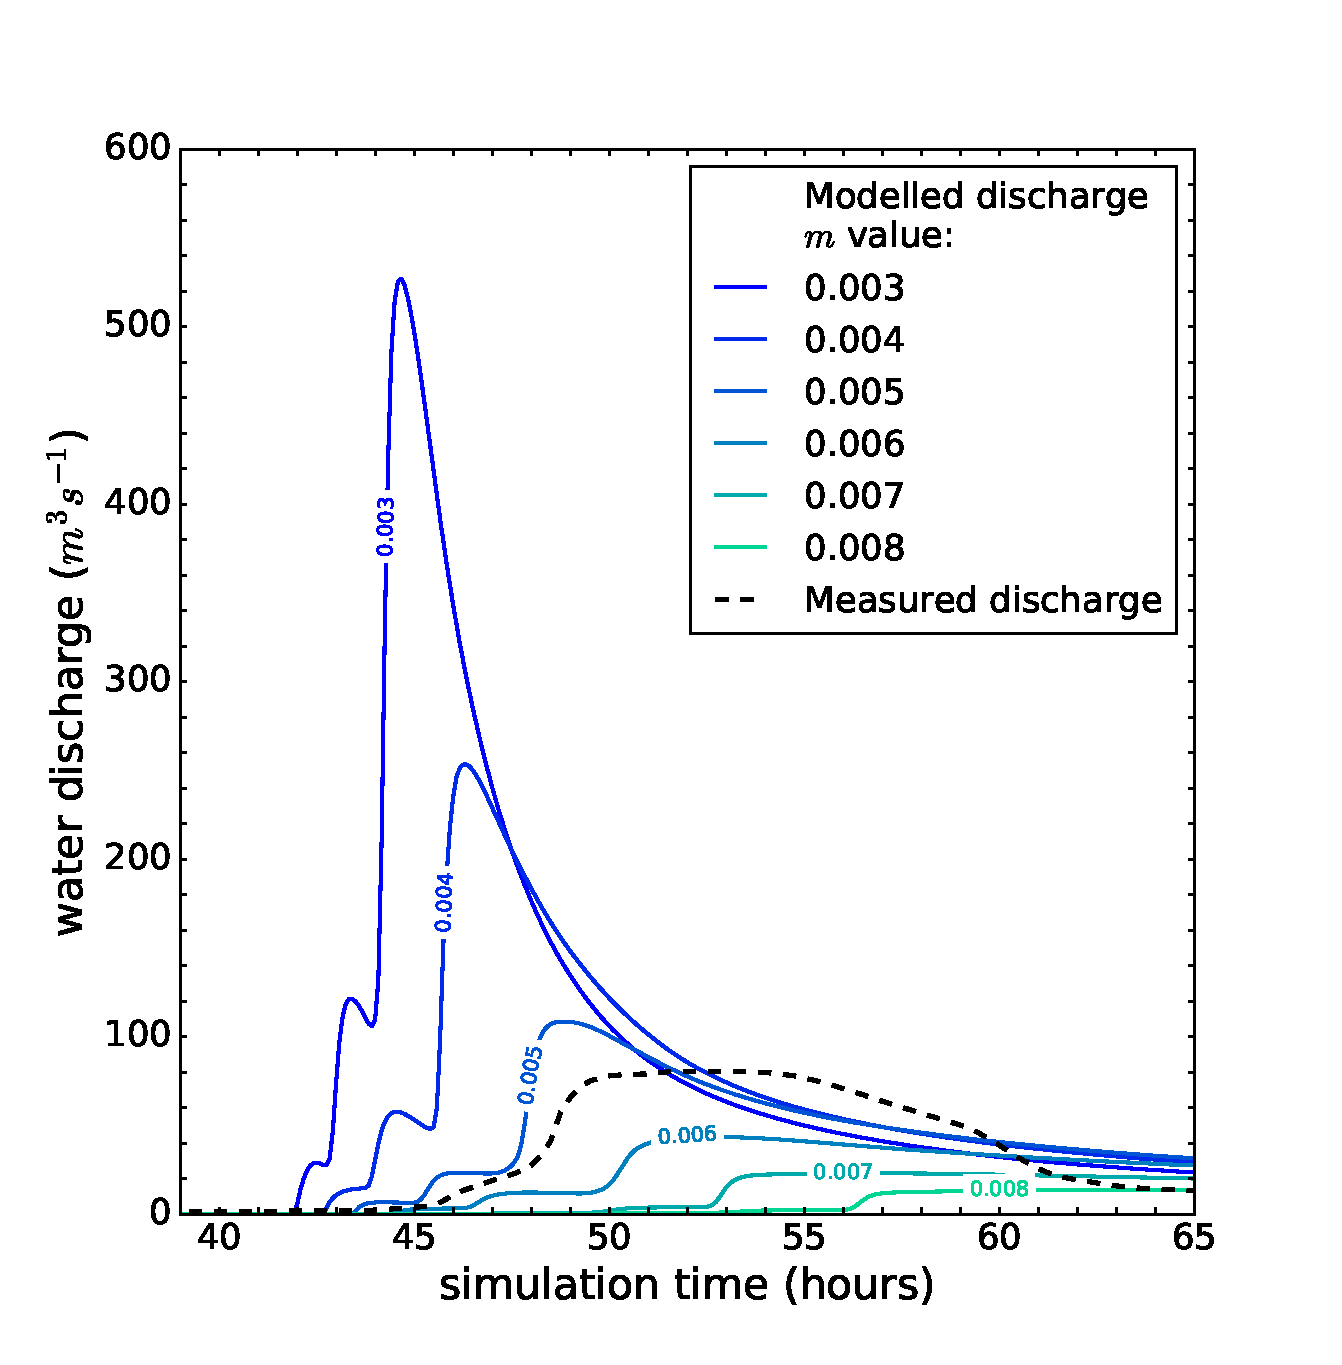
\includegraphics[width=11cm]{chp06_figures_scripts/figure_ryedale_M_sens.eps}
\caption{Discharge at Ryedale catchment outlet for varying values of the TOPMODEL \(m\) parameter. The measured discharge at the catchment gauging station is overlain in dashed line. The results from the simulations with \(m\) \textgreater \ 0.008 are omitted for clarity due to the low peak discharges they produced.}
\label{fig_topmodel_m_ryedale}
\end{figure}

\subsection{Catchment hydrology}

%Comparisons with the actual hydrographs from the gauged basins?

At the catchment scale, hydrological response was sensitive to both the rainfall resolution and the choice of erosional model. For both catchments, higher resolution rainfall input data resulted in a greater maximum river discharge. In the Ryedale experiments, simulations using the gridded rainfall input experienced a flashier hydrological response, reaching peak discharge several hours before the uniform rainfall input cases. This was not observed in any of the Boscastle simulations, with all simulations reaching peak discharge within 30 minutes of each other.

The choice of erosion model also influenced the hydrological response. When catchment erosion was modelled using a transport-limited case, peak discharges were higher in all cases, but the timing of hydrograph peaks remained similar for each case. The difference in peak discharges were minimal when comparing the detachment-limited cases to the hydrological-only models.

\begin{figure}[t]
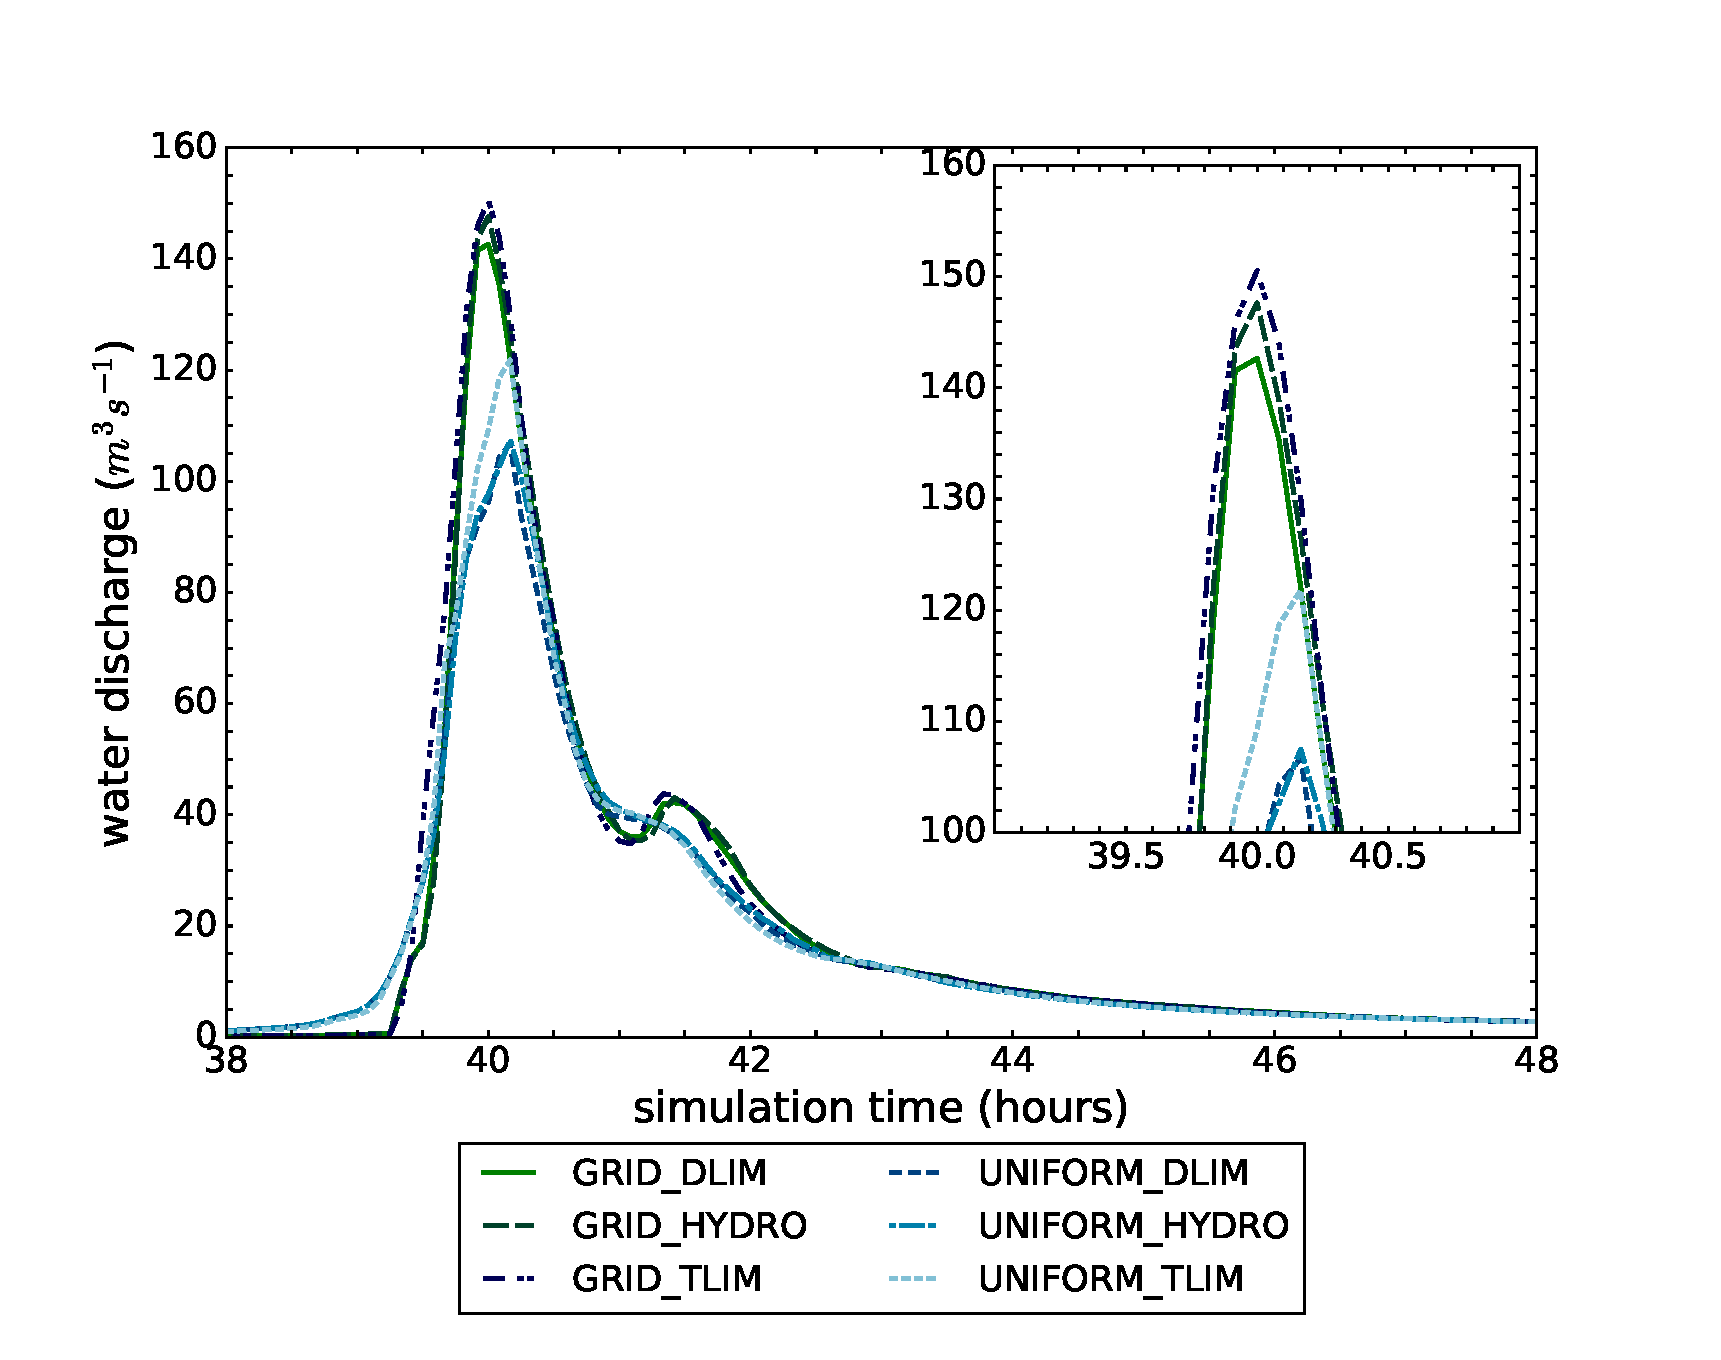
\includegraphics[width=14cm]{chp06_figures_scripts/figure_boscastle_hydrograph_ensemble.eps}
\caption{Boscastle hydrographs (discharge over time at catchment outlet) for each simulation of the 2004 Boscastle event listed in Table \ref{table_ensemble_experiments}. Inset shows detail of main flood peaks around hour 40 of the simulation.}
\label{fig_boscastle_hydrograph_ensemble}
\end{figure}

\begin{figure}[t]
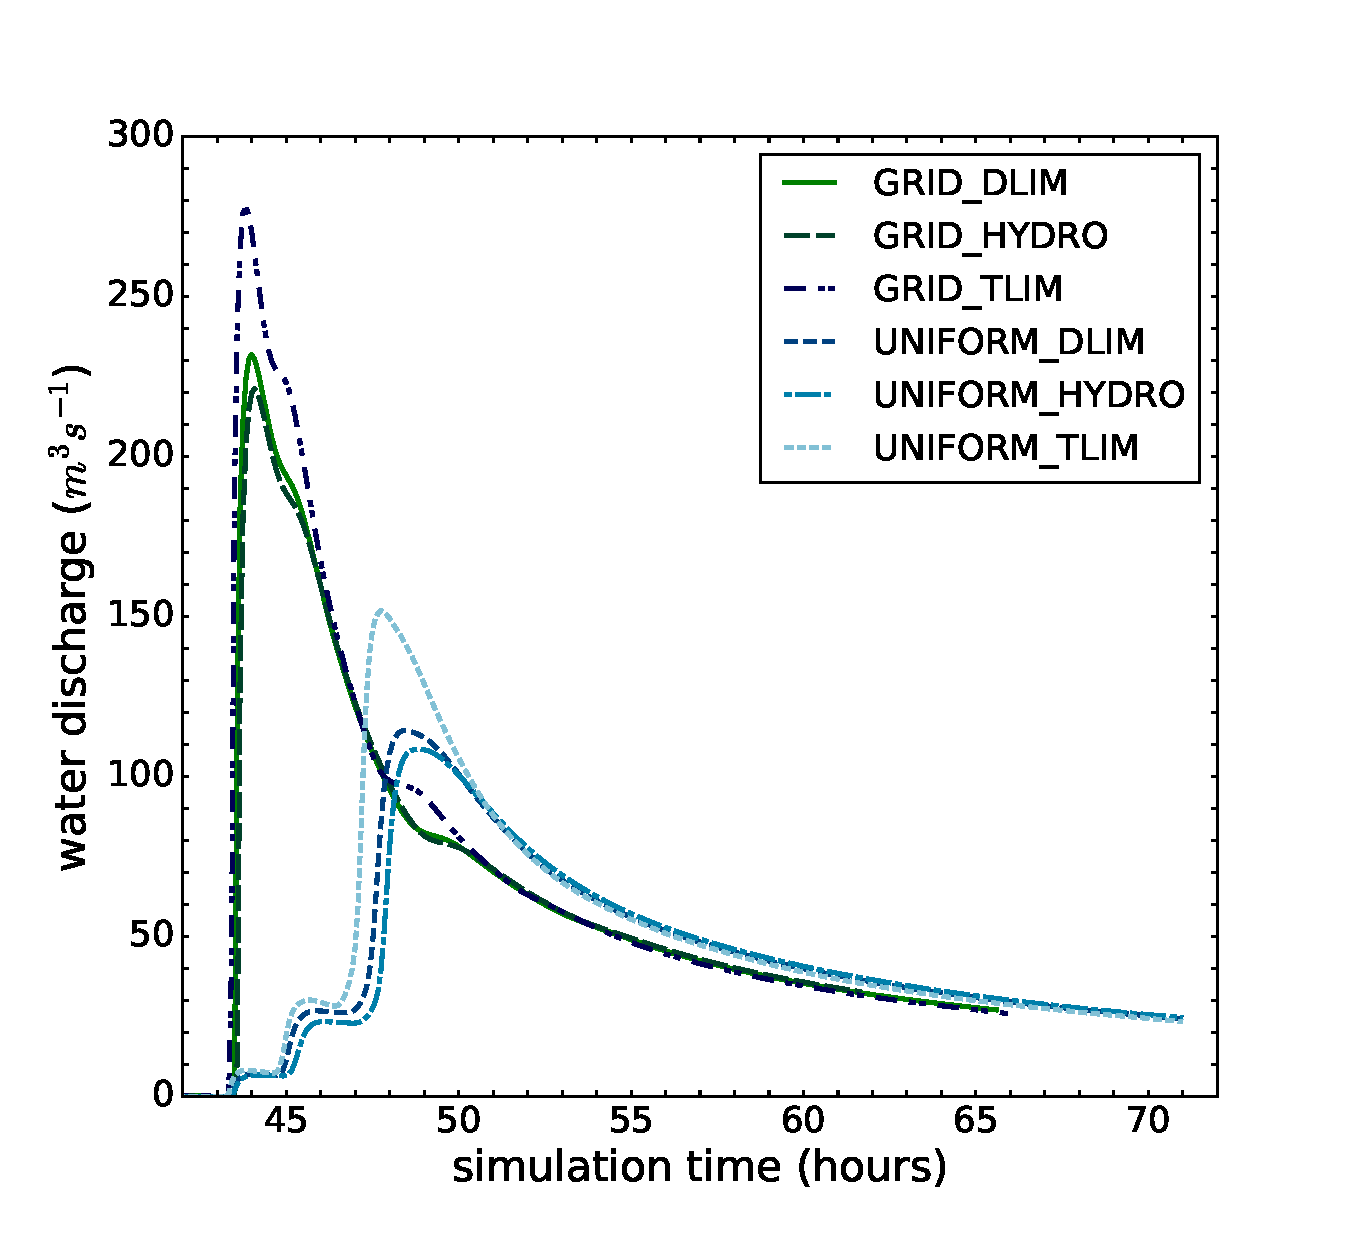
\includegraphics[width=14cm]{chp06_figures_scripts/figure_ryedale_hydrograph_ensemble.eps}
\caption{Ryedale hydrographs (discharge over time at catchment outlet) for each simulation of the 2005 Ryedale event listed in Table \ref{table_ensemble_experiments}.}
\label{fig_ryedale_hydrograph_ensemble}
\end{figure}



\subsection{Spatial variation in flood inundation}
\subsubsection{Boscastle}
The Boscastle catchment simulations showed minimal variation in flood inundation extent. Simulations with gridded rainfall input did not result in substantially different predictions of floodwater inundation compared to those with uniform rainfall input. Both sets of simulations reflected the general extent of reported flood water extents (Cite Engineers Report XXXX). Simulations that allowed erosion to take place (GRID\_TLIM and UNIFORM\_TLIM) showed a slight difference in the variation of floodwater depths in the floodplain area, particularly in the vicinity of Boscastle village, where Figure \ref{fig_boscastle_2dplan_flood_ensemble} is centred on. In hydrological-only simulations, the deepest water depths were predicted to occur in the confines of the river channel, whereas in erosion-enabled simulation, there appeared to be a `smoothing' effect of water depths between the channel and the adjacent floodplain, suggesting that the channel geometry had altered during the flood event either by infilling from sediment from upstream or collapse of the adjacent river banks. Engineer's reports of the Boscastle flood noted that the river channel in the Boscastle village area had indeed been inundated with debris during the storm, which had potentially contributed to the extent of the flooding within the village.

\subsubsection{Ryedale}
The Ryedale simulations showed greater variation in flood extent between the gridded rainfall and uniform rainfall inputs. The flood extents were greater in the gridded rainfall input simulations, corresponding with the higher peak discharges predicted in these simulations.  The variation in water depths appeared to be less sensitive in comparison to the Boscastle simulations. In the lower reaches of the catchment (Figure \ref{fig_ryedale_2dplan_flood_ensemble}, there appeared to be little indication that flood extents or water depths were sensitive to the erosion parameterisation, in contrast to the Boscastle simulations.



% Plan view erosion diff maps
\begin{sidewaysfigure}[t]
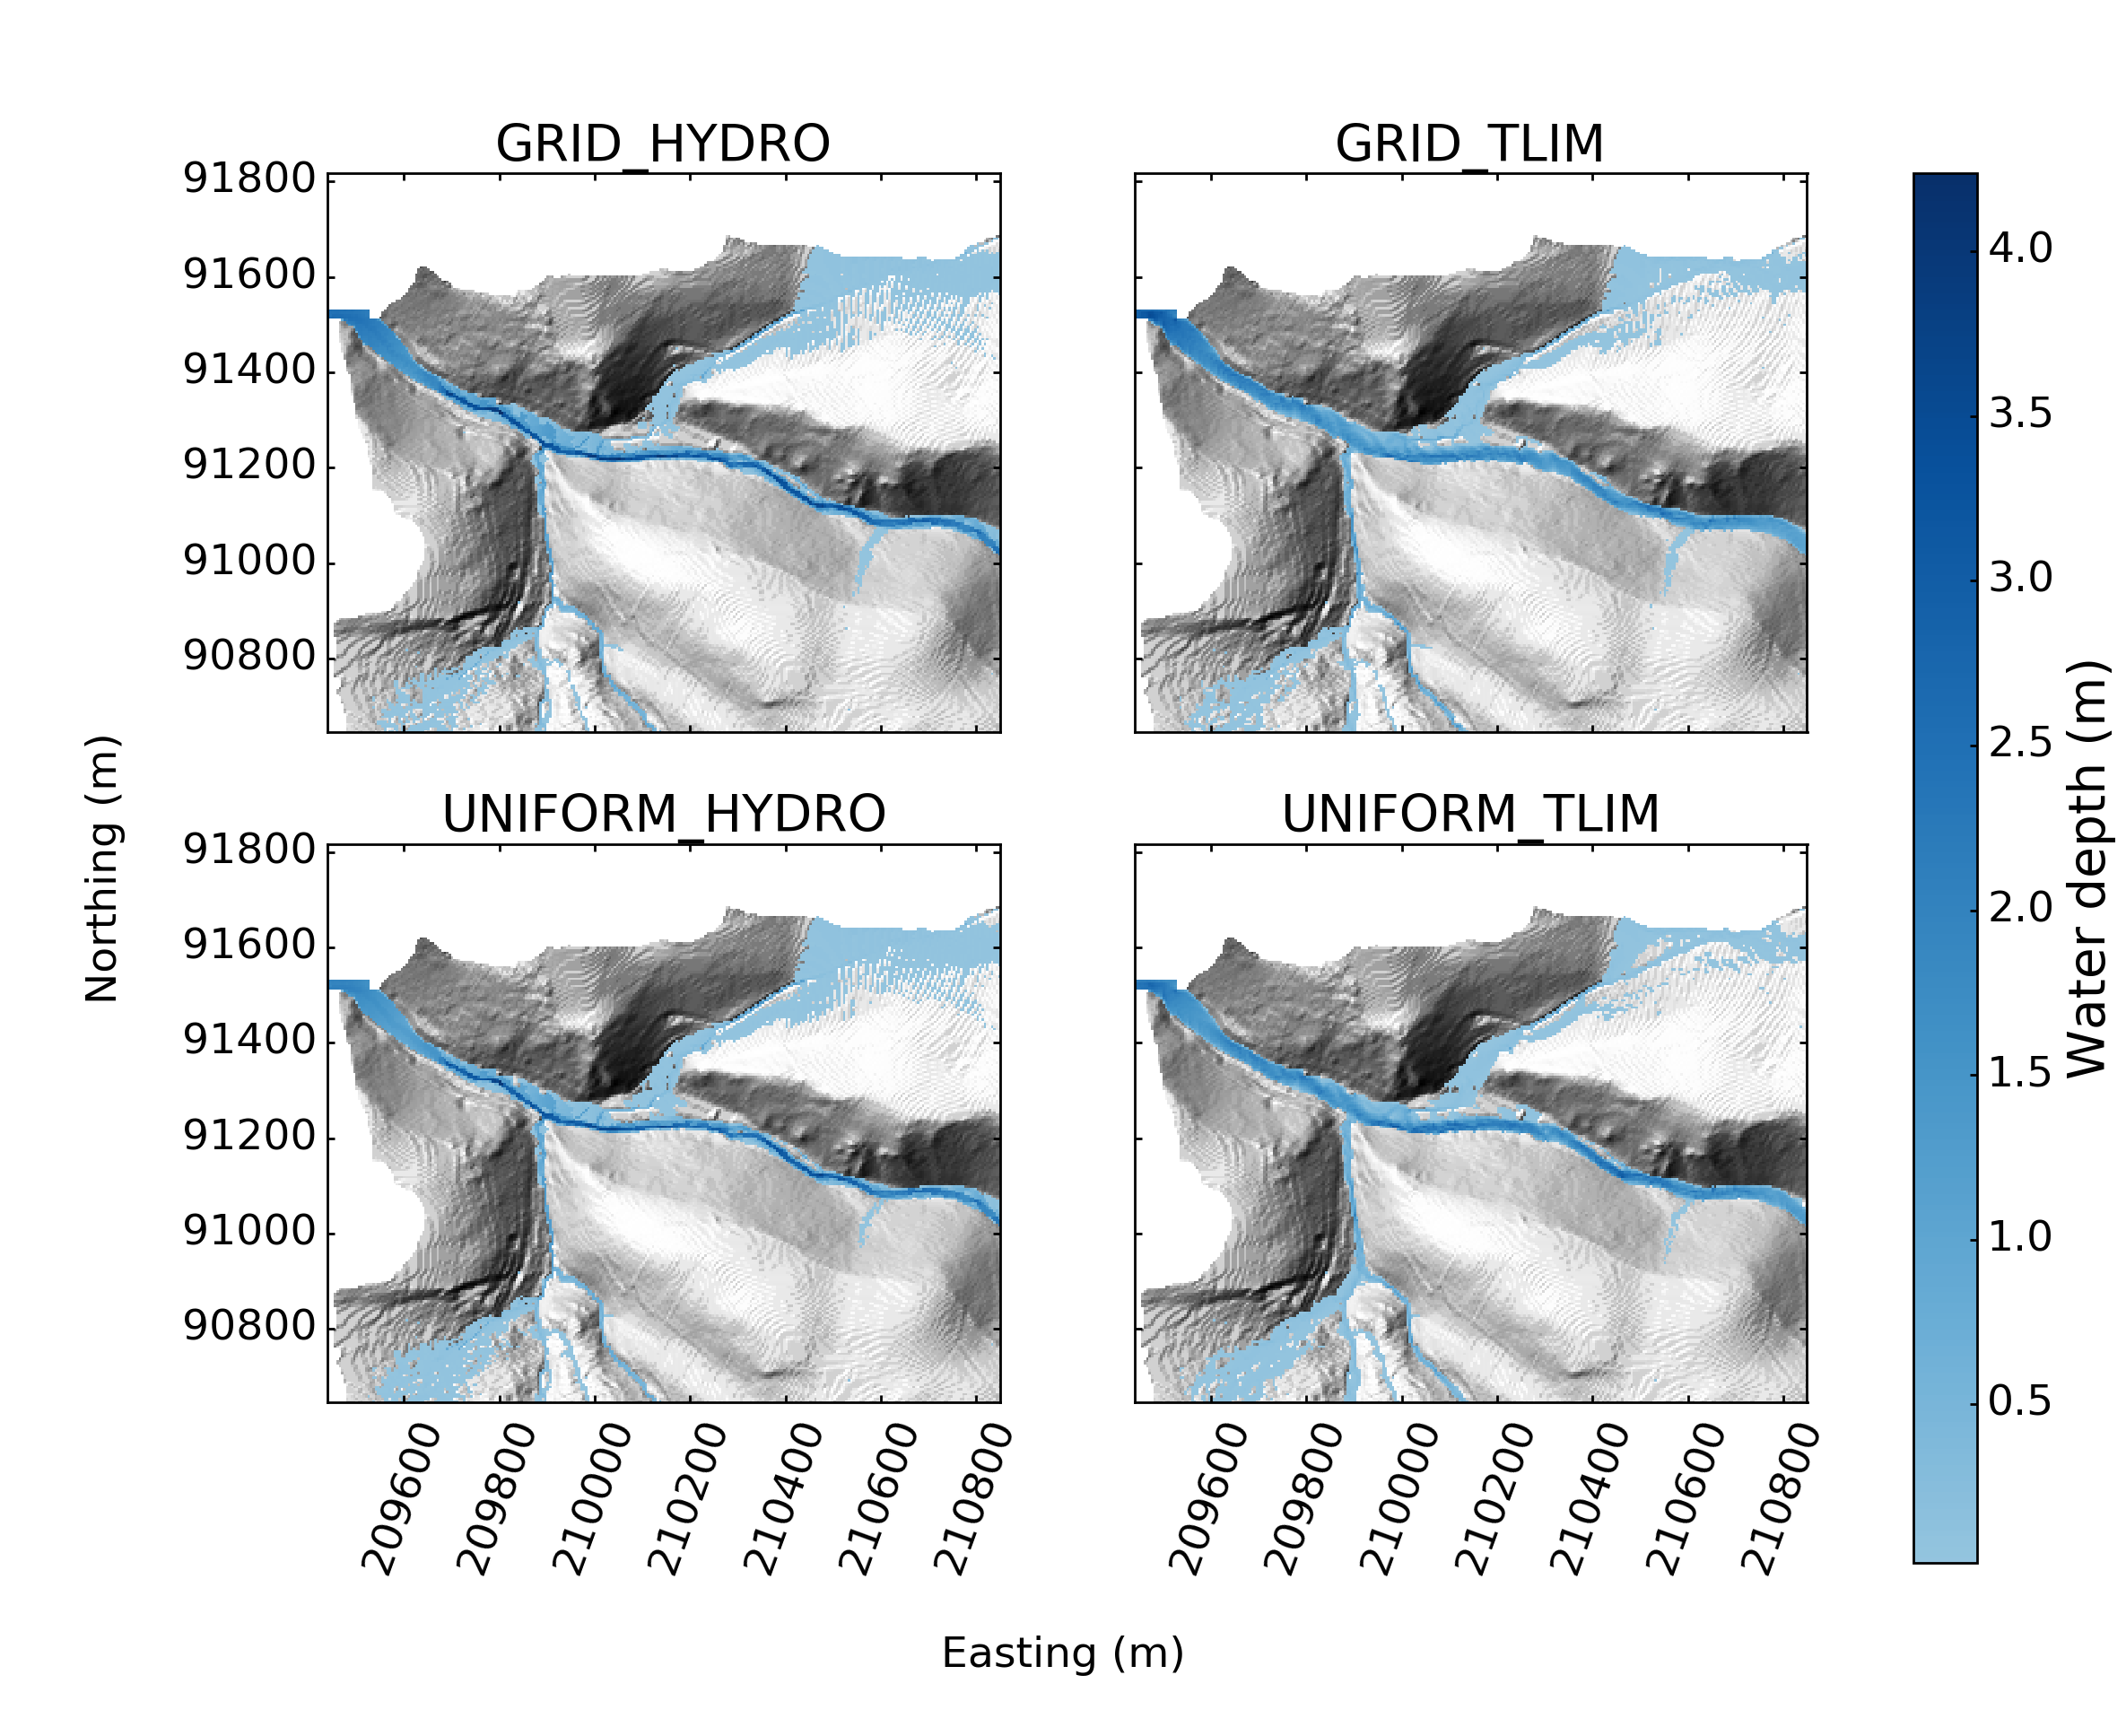
\includegraphics[width=20cm]{chp06_figures_scripts/figure_boscastle_peak_flood_ensemble.png}
\caption{Flood extents in the Boscastle catchment at the time of maximum river discharge for each simulation.}
\label{fig_boscastle_2dplan_flood_ensemble}
\end{sidewaysfigure}

% Plan view erosion diff maps
\begin{sidewaysfigure}[t]
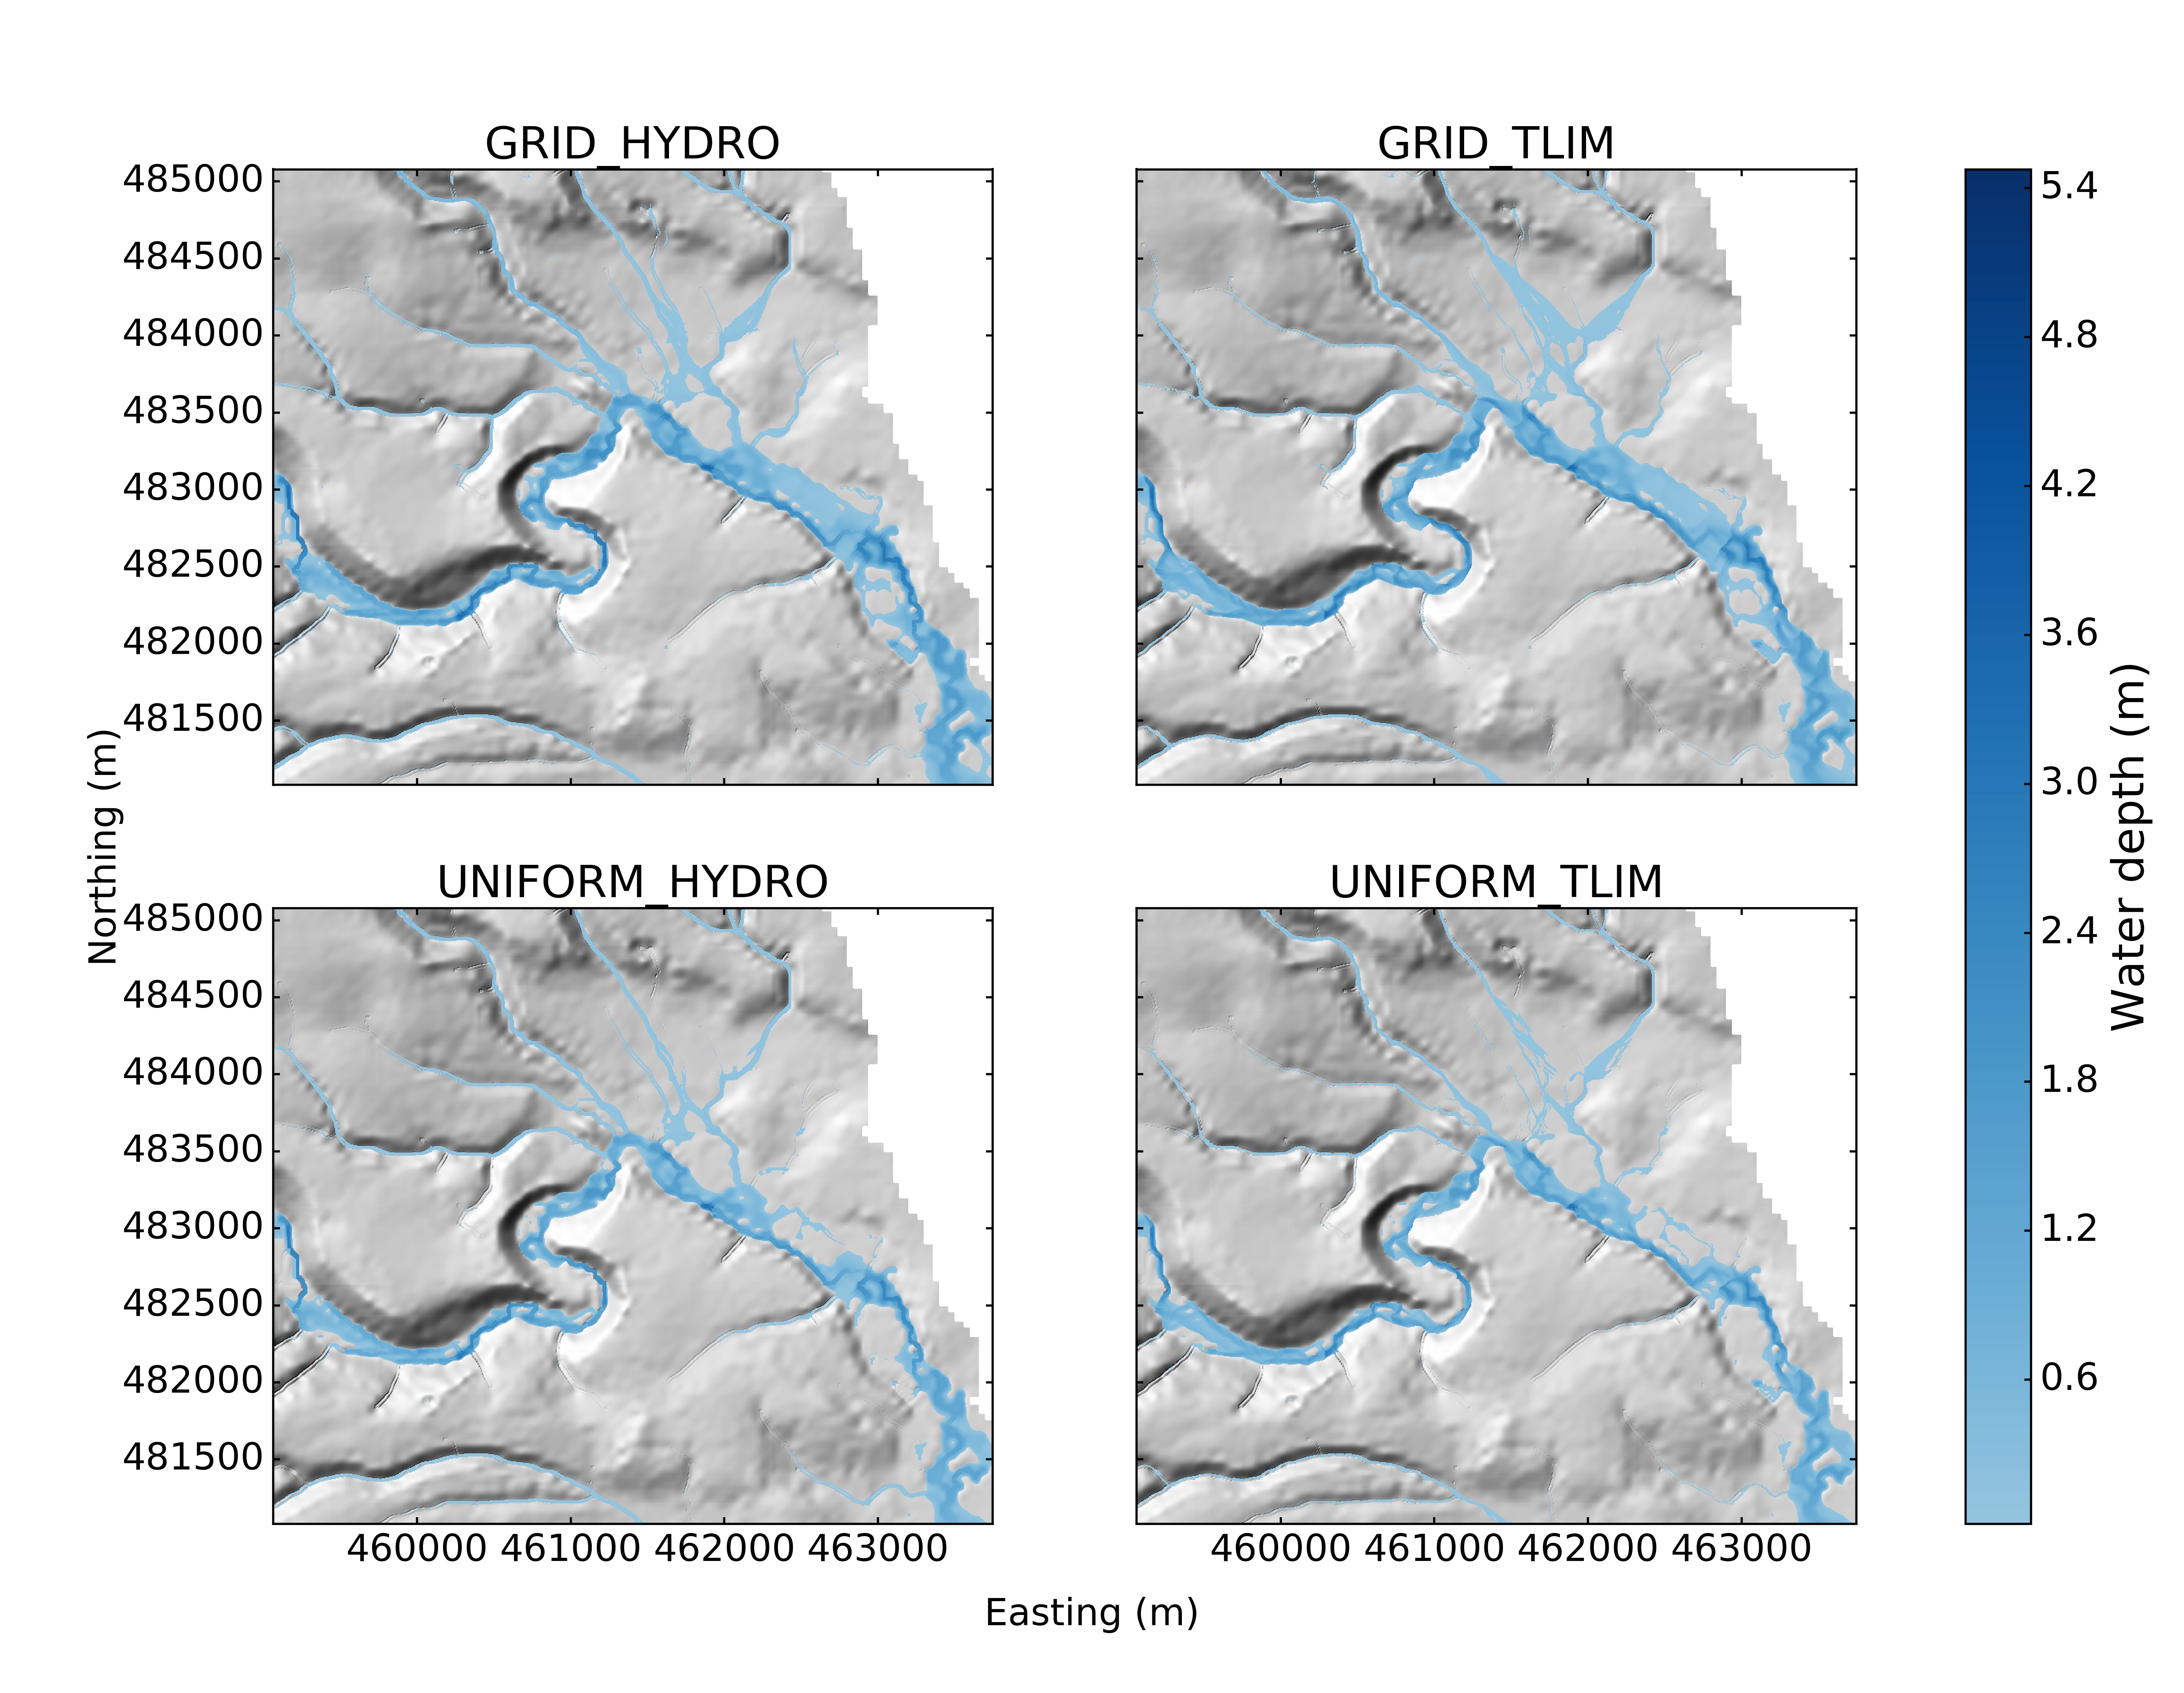
\includegraphics[width=20cm]{chp06_figures_scripts/figure_ryedale_peak_flood_ensemble.png}
\caption{Flood extents in the Ryedale catchment at the time of maximum river discharge for each simulation.}
\label{fig_ryedale_2dplan_flood_ensemble}
\end{sidewaysfigure}



\section{Discussion}


The size of the two catchments appears to be a determining factor in how sensitive hydrogeomorphic processes are to the rainfall data input resolution. The Boscastle catchment at 18 km\(^2\) is approximately an order of magnitude smaller than the Rydedale catchment at 270 km\(^2\). For each simulation using gridded rainfall input, the cell width of the rainfall grid is 1 km. The relative amount of increase in rainfall detail between uniform and gridded simulations is much greater in the larger Ryedale catchment than the Boscastle catchment. By using a 1 km gridded rainfall product as input data, the Ryedale simulation potentially captures 15 times more rainfall heterogeneity compared to the respective Boscastle simulation, by virtue of it simply being a much larger catchment with a greater number of rainfall input cells. Catchment size is known to be a factor in hydrological studies of rainfall resolution, and larger catchments are reported to show greater sensitivity to rainfall resolution \citep[e.g.][]{nicotina2008impact}, in terms of hydrological response.

Increasing the resolution of rainfall input data may not be enough to observe sensitivity in smaller catchments, as rainfall features themselves may not exhibit the necessary heterogeneity in structure to benefit from being resolved at finer scale. Rain cells or bands equal to or greater in size than the catchment over which they rain upon, may well be homogeneous enough in spatial extent and rainfall rate that a `uniform' approximation of their rainfall rate is sufficiently precise enough to represent the rainfall rate at all points in the catchment. As seen in the Boscastle catchment simulations, using a detailed rainfall input data source did not notably alter the outcome of the hydrological predictions (Figures \ref{fig_boscastle_2dplan_flood_ensemble}, \ref{fig_ryedale_2dplan_flood_ensemble}). In the Ryedale catchment simulations, the hydrological predictions were notably different based on the choice of rainfall input data resolution, affecting both the time and magnitude of the resulting flood peak. 

Talk about size of convective cell features. What is typical storm cell size and heterogeneity (decay from centre?).

\subsection{Implications for longer-term landscape evolution}
The experiments presented in this chapter have focused on the hydrogeomorphic response to single severe storm events, events which produced floods with return periods of 1 in 330 years (Ryedale) and 1 in 1300 years (Boscastle). The amounts of river channel incision predicted as a result of these storms is comparable to that predicted by studies of landscape evolution on scales of 1000 years, for example a study of a similar upland river basin by \citep{coulthard2016sensitivity} predicted channel incision amounts of 0.5--5m over 1000 years. The experiments presented here, using the same sediment transport law, predicts comparable incision amounts of channel incision during a single storm. If the flood return periods are assumed to be broadly correct, these simulations suggest that the majority of sediment erosion occurs during rare but high magnitude flood events, rather than through gradual processes or more frequent but lower magnitude events.

%%%%%%%%%%%%%%%%%%%%%
\section{Conclusions}  %% \conclusions[modified heading if necessary]
%%%%%%%%%%%%%%%%%%%%%
Over long term landscape evolution, erosional proccesses in catchments are known to be sensitive to the spatial distribution of rainfall input. Catchment hydrological response on the short term scale -- such as during the course of single storm event -- is also sensitive the spatial input pattern of rainfall, with the simulations carried out in this study also supporting similar work of \citep{nicotina2008impact} AND OTHERS. This study has shown that catchment erosional processes are also sensitive to rainfall spatial distribution during the course of a single severe storm, and it is suggested that this is due to the spatial variation in shear stresses required brought on by heterogeneous rainfall inputs to the catchment system.  As sediment transport and erosional process are highly threshold dependent, this leads to erosional patterns that differ according to the pattern of rainfall input. In other words, in the simulation of landscape evolution processes at the catchment scale, the choice of whether to use a uniform value representing the rainfall input, or to use a spatially heterogeneous gridded rainfall data, can have a marked impact on the predicted sediment yields from the catchment, as well as slight variations in the prediction flood inundation extents and the timing of peak flood levels.

In terms of sediment yields, however, these experiments have shown that it is the choice of erosional parameterisation in the model, and not necessarily the resolution of rainfall input data, that has a first-order control on the total sediment yields from a catchment and the magnitude of river channel incision during a simulated event.

Stuff amount rarity of events. Catastrophism.


\section{Fixed parameters}

\textit{A table showing the other parameters used in the simulations (All of which remain fixed for each simulation)}

The following table lists the parameters that were held constant for all simulations.
